%% marcel's template

\documentclass[12pt]{article}
\usepackage[margin=0.5in]{geometry}
\usepackage{amsmath,amsthm,amssymb,amsfonts,tikz,tikzsymbols}
\usepackage[shortlabels]{enumitem}

\usepackage{float}% for making figures behave with H

\usepackage{hyperref}
\hypersetup{
  colorlinks   = true,    % Colours links instead of ugly boxes
  urlcolor     = blue,    % Colour for external hyperlinks
  linkcolor    = blue,    % Colour of internal links
  citecolor    = red      % Colour of citations
}

\newenvironment{rcases}
  {\left.\begin{aligned}}
  {\end{aligned}\right\rbrace}

\newcommand{\N}{\mathbb{N}}
\newcommand{\Z}{\mathbb{Z}}
\newcommand{\Q}{\mathbb{Q}}
\newcommand{\R}{\mathbb{R}}
\newcommand{\C}{\mathbb{C}}
\newcommand{\F}{\mathbb{F}}
\newcommand{\RA}{\Rightarrow}
\newcommand\defeq{\mathrel{\stackrel{\makebox[0pt]{\mbox{\normalfont\tiny def}}}{=}}}

\newcommand{\M}{\mathbb{M}}

\renewcommand\qedsymbol{$\Smiley$}

\newenvironment{problem}[2][Question]{\begin{trivlist}
\item[\hskip \labelsep {\bfseries #1}\hskip \labelsep {\bfseries #2.}]}{\end{trivlist}}
\newenvironment{exercise}[2][Exercise]{\begin{trivlist}
\item[\hskip \labelsep {\bfseries #1}\hskip \labelsep {\bfseries #2.}]}{\end{trivlist}}
%If you want to title your bold things something different just make another thing exactly like this but replace "problem" with the name of the thing you want, like theorem or lemma or whatever

\begin{document}
 
%\renewcommand{\qedsymbol}{\filledbox}
%Good resources for looking up how to do stuff:
%Binary operators: http://www.access2science.com/latex/Binary.html
%General help: http://en.wikibooks.org/wiki/LaTeX/Mathematics
%Or just google stuff
 
\title{\texttt{DATA\_SILSO\_HISTO}\\Quality Control Report}
\author{Stephen Fay}
\maketitle

\tableofcontents

\section{Introduction}
\subsection{Github repository and project}
    https://github.com/dcxSt/DATA\_SILSO\_HISTO\_search \\
    https://github.com/users/dcxSt/projects/2?fullscreen=true
    
\subsection{Brief History et Mise en Contexte}

For centuries we have observed the sun and it's ever mysterious sunspots. The 11 year sunspot cycle has long been a subject of debate. Today we wish to have precise quantification of solar activity throughout the previous centuries. This is made possible by the sunspot series. For the past 3 to 4 hundred years people all over the Eurasian continent have been recording the number of sunspots that appear on the sun's earth facing half. 

The aim of this project is to do a quality control of the data in DATA\_SILSO\_HISTO. Once the data is fixed and cleaned up, it will be stored on a new database - temporarily named GOOD\_DATA\_SILSO in a more user-friendly format to what currently exists. I will also get rid of any useless or redundant columns (such as the observers comment column - there are no comments )': ). A third, temporary database will be mad to keep a closer eye on the data that still needs to be examined with more scrutiny : BAD\_DATA\_SILSO. This database will act as intermediary between DATA\_SILSO\_HISTO and GOOD\_DATA\_SILSO. We will effectively be storing 2 databases-worth of information in 3 databases. The original DATA\_SILSO\_HISTO will have the old data and will be corrected in due course. The intermediary BAD\_DATA\_SILSO will start as a copy of DATA\_SILSO\_HISTO and end up empty as the corrected data is removed from it and placed, in the new format, into GOOD\_DATA\_SILSO.


\section{Setup}

\subsection{What do the flags mean?}\label{flags section}
\newpage% idk how to make tables behave!
\begin{table}[H]
    \centering
    \begin{tabular}{c|c|c|c|c}
        0 & 1 & 2 & 3 & 4 \\
        same as Null & suspicious & Comment in journal = ? & move to bin & suspiciously high\\
        \hline
        5 & 6 & 7 & 8 & 9\\
        v. suspiciously high & misc see comment & derived from area-measurements & mauvaise def & null sunspots
         
    \end{tabular}
    \caption{Flags key}
    \label{tab:flag}
\end{table}

\begin{enumerate}[start=0]
    \item The default for the flag is NULL, when is estimate that the datapoint is perfect and there is nothing wrong with it, I can put it to zero 0.
    \item If the data looks fishy but I'm not quite sure either what is wrong with it or how wrong it is this is flagged with a 1 - the default.
    \item If in the Mitteilungen journals there is written a `?' next to one of the data points, I will mark it with a 2, this means that the observer is not quite confident in his/her result. See \ref{what is flag 2 question mark} - July 3 for speculation on what I think comment `?' means.
    \item A flag that signifies that this data point is definitely going into the bin
    \item For data that is very dodgy but it is ambiguous as to weather or not it is correct, to determine its validity closer examination is required
    \item For data that is very dodgy, the difference between 5 and 4 is illustrated by example: if i find that a datapoint has a groups number of 30 I will mark it with a 4 and comment it, because this is suspicious, if a datapoint has a groups number over 60 or above, it will be marked with a 5 (trust me there are some in the hundreds). When it comes to sunspots it's the same but with 100 for 4 and 250 for 5
    \item Miscellaneous data, take a look at the comment, often the comments here will be what is written in the Mittheilungen.
    \item Data who's values have been derived from some formulae, usually because observer noted down area measurements of the total number of millimeters the sun-disk was taken up by sunspots.
    \item Bad definition of the sun picture
    \item No sunspots numbers indicated.
\end{enumerate}


\subsection{Equations}

\begin{equation}\label{derivde equation}
    r = a\cdot(10 g + b\cdot f) = 10 a\cdot g + c\cdot f
\end{equation}

\begin{equation}\label{standard deviation equation}
    \sigma = \sqrt{\frac{\sum_{i=1}^{n} (x_i - \bar{x})^2}{n-1}}  \quad \quad \quad \quad 
    var = \frac{\sum_{i=1}^{n} (x_i - \bar{x})^2}{n-1}
\end{equation}

Since we have models where $\bar{x}$ is not the mean but a linear model
\begin{equation}\label{standard deviation percentage equation}
    \sigma\% = 100\cdot \sqrt{\frac{\sum_{i=1}^{n}\big(\frac{x_i-\bar{x}}{\bar{x}}\big)^2}{n-1}}
\end{equation}


\subsection{Python scripts - what they contain}

See README.md - it is automatically generated based on what are in the scripts. Generated by the file \texttt{create\_readme.py}

\section{Condensed Log}

\subsubsection{Before The Solstice}
I only started the log on the solstice so I forgot the details of what I was doing before then. The time was spent learning the basics of \texttt{SQL} and how to interface with an \texttt{SQL} database through the mysql terminal; acquainting myself with the data and with what it is I ought to be doing. This is the period where I wrote some of the basic methods that I now use every day for accessing and connecting with the Mittheilungen.

\subsubsection{Friday June 21}
\begin{itemize}
    \item Started writing the log
    \item Made `searching\_the\_manuals.py'
    \item Searching database for `uncertain' comments
\end{itemize}
    
\subsubsection{Monday June 24}
\begin{itemize}
    \item Discovered and sorted a bunch of duplicate data, two data-points for one date and one observer
    \item Methods used can be found in \texttt{searching\_the\_manuals.py}
\end{itemize}
    
\subsubsection{Tuesday June 25}
\begin{itemize}
    \item Backed up the databases and started flagging for the moving process.
    \item Wrote a new script to deal uniquely with deleting the duplicates (and putting them into `\texttt{RUBBISH\_DATA}')
    \item Commented the rubbished duplicate data points
\end{itemize}
    
\subsubsection{Wednesday June 26}
\begin{itemize}
    \item Wrote methods for finer mass commenting (in \texttt{db\_edit.py})
    \item Flagged data with abnormally large groups and or sunspots numbers. (FLAG=4 WHERE $>$ 100 ; FLAG=5 WHERE $>$ 250)
    \item Set 212 flags 3 for putting things in the bin. There are still 4000 pairs of duplicates that need attending to, originally there where 14000
    \item Scrutinised what I had flagged, reread my scripts, checked that things are in the right place.
    \item Having doubts about what is reasonable / unreasonable sunspots number.
\end{itemize}
    
\subsubsection{Thursday June 27}
\begin{itemize}
    \item Scrutinised flagged data from yesterday
    \item Turned my attention to the data labeled `*' in the comments
    \item Moved the flagged duplicates to \texttt{RUBBISH\_DATA}
    \item Found many instances of data written in wrong year
    \item Started writing \texttt{corrections\_needed\_handwritten.txt}, to make clear all my tasks.
\end{itemize}
    
\subsubsection{Friday June 28} 
\begin{itemize}
    \item The notes I took about the duplicates can be found in different\_value\_duplicates.txt, some things I found interesting so I decided to copy most of the file into this report (see long log)
\end{itemize}
    
\subsubsection{Monday July 1}
\begin{itemize}
    \item Using what I did on Friday to bin some duplicated data and modify some other data
    \item Made a new alias in \texttt{DATA\_SILSO\_HISTO} (and \texttt{BAD\_DATA\_SILSO}) called `Brunner Assistent'.
    \item Backed up the the databases to sql files
    \item Most of this data has been cleaned up, the rest can be done by hand
\end{itemize}
    
\subsubsection{Tuesday July 2}
\begin{itemize}
    \item Made some pretty plots in \textit{suspicious sunspots plots.ipynb} in the root directory
    \item Made a method in the jupyter notebook mentioned above that plots an observer's stuff and color codes the flags.
    \item Checked some of them in the journals
    \item Started patching Tacchini's missing holes
\end{itemize}
    
\subsubsection{Wednesday July 3}\label{what is flag 2 question mark}
\begin{itemize}
    \item Continued fixing Tacchini (see figure \ref{fig:tacchini})
    \item Went back to searching the manuals for errors from error sheet. 
    \item Looking through for `uncertain' comments
    \item Figured out what COMMENT=`?' means; blurry image / bad definition of img
    \item Found some comments where there is both an observer and a question mark at the same time, for these ones I left the comments as they are and changed only the flag from 1 to 2.
    \item Finished looking at red comments (I still need to change them and move them all with python, I will do it tomorrow.) 
    \item Looking at blue comments (the ones where comments are just numbers)
    \item Backed up databases
    \end{itemize}
            
\subsubsection{Thursday July 4}
\begin{itemize}
    \item Looking into Carrington's case.
    \item I updated the flag 7 to ``derived from area-measurement" and flagged all of Secchi's sunspot values that were derived from the penumbra and / or umbra.
    \item Dealt with Secchi
    \item Spoke to F. Clette about the possible conversion from the `aire' to a sunspots number. He gave me some clues as to where to look in the mitt.
    \item Excitement! I found on page 131 of Mitt 31-40 written after rubrics 299 a description of how the author (I think R. Wolf himself) derived a formula for turning Secchi's `aire' into a sunspots number
    \item \ref{converting the `aire'} here is what is written in German and Italian, with a translation in English.
    \item Backed up databases
\end{itemize}
        
\subsubsection{Friday July 5}
\begin{itemize}
    \item Continued working on Carrington - Main event = did a least-squares regression fit to optimise the constant values in the equation that transforms `aire' into wolf number.
\end{itemize}

\subsubsection{Monday July 8}
\begin{itemize}
    \item Finished deriving Carrington
    \item Backed up databases
\end{itemize}

\subsubsection{Tuesday July 9}
\begin{itemize}
    \item Derived Kew's misbehaving data
    \item Made a new `README.md' that auto-generates based on what is inside my python scripts
    \item Tidied the report and added some figures
\end{itemize}

\subsubsection{Wednesday July 10}
\begin{itemize}
    \item Sabrina gave Arnaud and I a tour of the Observatories facilities
    \item Separated Carrington into two aliases
    \item Figured out what to do with Secchi (now I just have to do it)
\end{itemize}

\subsubsection{Thursday July 11}
\begin{itemize}
    \item Dealt with rubrics 375, see \texttt{secchi\_derivation.ipynb}
    \item Dealt with 2 more of Secchi's rubrics, there are still 2 annoying ones
    \item Continued checking and correcting typos and anomalies from the blue comments sheet
\end{itemize}

\subsubsection{Friday July 12}
\begin{itemize}
    \item Dealt with the red comments, changed alot of their comment to `?' which was written in the journals and changed the flag to 2
    \item Put some thought into how to deal with oranges aswell as Wolf / Wolfer
\end{itemize}

\subsubsection{Monday July 15}
\begin{itemize}
    \item Transferred all the data with flag = 2 into the database \texttt{GOOD\_DATA\_SILSO}
    \item Upgraded the plotting methods in \texttt{graphs\_helper.py}
    \item Plotted Wolf and Wolfer and aliases in which they appear - see \texttt{wolf\_wolfer\_investigation.ipynb}
    \item Brainstormed how I was gonna tackle wolf / wolfer's data
\end{itemize}

\subsubsection{Tuesday July 16}
\begin{itemize}
    \item Planned out how I was going to tackle the Wolf - Wolfer problems
    \item Wrote some methods to smooth data and also to plot the sunspots number
    \item Corrected typos and errors
\end{itemize}

\subsubsection{Wednesday July 17}
\begin{itemize}
    \item Corrected Adam's data by hand data-point by data-point
    \item Made some more plots in the \texttt{wolf\_wolfer\_investigation.ipynb}
    \item Investigated Wolfer some more
    \item Accidentally deleted database and lost all the edits I made to the database today... :(  [luckily I have backups from yesterday]
\end{itemize}

\subsubsection{Thursday July 18}
\begin{itemize}
    \item Accidentally deleted the data again, re-corrected Adam's data by hand
    \item Fixed the data and imported the old data into the database \texttt{ORIGINAL\_DATA\_SILSO\_HISTO}
    \item Wrote to Laure and she gave me some good ideas for how to detect drift
    \item Rereading papers to get better understanding of what I ought to be doing
\end{itemize}

\subsubsection{Friday July 19}
\begin{itemize}
    \item Made a cool plotting tool in an attempt to visualise the drift of observers, didn't work out brilliantly
    \item Made a couple new aliases which I populated with data `Mooser' (for rubrics 122 only)
    \item Made the alias `Wolfer P' who now has 307 datapoints.
\end{itemize}

\subsubsection{Monday July 22}
\begin{itemize}
    \item Wrote a cute little script to automate backing up the databases.
    \item Translated a big long rubrics
    \item Sorted all the data attached to fk\_observers IN (60,61,62) - all composite observers from these strange rubrics\_number = 0 in the mid to late 1800's - into their proper observers.
\end{itemize}


\section{Tables & Figures}

\subsubsection{The original sql data tables format}

\begin{table}[h!]
    \centering
    \caption{DESCRIBE DATA}
    \begin{tabular}{c|c|c|c|c|c}% l c r = Left Centre Right
        \textbf{Field} & \textbf{Type} & \textbf{Null} & \textbf{Key} & \textbf{Default} & \textbf{Extra}  \\
        \hline
        ID & int(11) & No & PRI & NULL & auto\_increment \\
        
        DATE & date & YES && NULL & \\
        
        FK\_RUBRICS & int(11) & YES & MUL & NULL &  \\
        
        FK\_OBSERVERS & int(11) & YES & MUL & NULL &  \\
        
        GROUPS & int(11) & YES && NULL &  \\
        
        SUNSPOTS & int(11) & YES && NULL & \\
        
        WOLF & int(11) & YES && NULL &  \\
        
        QUALITY & int(11) & YES && NULL &  \\
        
        COMMENT & text & YES && NULL &  \\
        
        DATE\_INSERT & datetime & YES && NULL &  \\
        
        FLAG (i added this) & tinyint(1) & YES && NULL &  \\
        
    \end{tabular}
    \label{tab:data-og}
\end{table}

\begin{table}[h!]
    \centering
    \caption{DESCRIBE OBSERVERS}
    \begin{tabular}{c|c|c|c|c|c}% l c r = Left Centre Right
        \textbf{Field} & \textbf{Type} & \textbf{Null} & \textbf{Key} & \textbf{Default} & \textbf{Extra}  \\
        \hline
        ID & int(11) & NO & PRI & NULL & auto\_increment \\
        
        ALIAS & varchar(50) & YES && NULL & \\
        
        FIRST\_NAME & varchar(50) & YES && NULL &  \\
        
        LAST\_NAME & varchar(50) & YES && NULL &  \\
        
        COUNTRY & varchar(50) & YES && NULL &  \\
        
        INSTRUMENT & varchar(50) & YES && NULL & \\
        
        COMMENT & text & YES && NULL &  \\
        
        DATE\_INSERT & datetime & YES && NULL &  \\
        
    \end{tabular}
    \label{tab:data-og}
\end{table}

\begin{table}[h!]
    \centering
    \caption{DESCRIBE RUBRICS}
    \begin{tabular}{c|c|c|c|c|c}% l c r = Left Centre Right
        \textbf{Field} & \textbf{Type} & \textbf{Null} & \textbf{Key} & \textbf{Default} & \textbf{Extra}  \\
        \hline
        RUBRICS\_ID & int(11) & NO & PRI & NULL & auto\_increment \\
        
        RUBRICS\_NUMBER & int(11) unsigned & NO && NULL & \\
        
        MITT\_NUMBER & int(11) unsigned & NO && 0 &  \\
        
        PAGE\_NUMBER & int(11) unsigned & YES && NULL &  \\
        
        SOURCE & text & NO && NULL &  \\
        
        SOURCE\_DATE & date & YES && NULL & \\
        
        COMMENTS & text & YES && NULL &  \\
        
        DATE\_INSERT & datetime & YES && NULL &  \\
        
        NB\_OBS & int(11) & YES && NULL & \\
        
    \end{tabular}
    \label{tab:data-og}
\end{table}

\newpage{}

\subsubsection{My new sql data table format}

\begin{table}[h!]
    \centering
    \caption{DESCRIBE DATA (the only table)}
    \begin{tabular}{c|c|c|c|c|c}% l c r = Left Centre Right
        \textbf{Field} & \textbf{Type} & \textbf{Null} & \textbf{Key} & \textbf{Default} & \textbf{Extra}  \\
        \hline
        ID & int(11) unsigned & No & PRI & NULL & auto\_increment \\
        
        DATE & date & YES && NULL & \\
        
        GROUPS & int(11) & YES && NULL &  \\
        
        SUNSPOTS & int(11) & YES && NULL & \\
        
        WOLF & int(11) & YES && NULL &  \\
        
        COMMENT & text & YES && NULL &  \\
        
        DATE\_INSERT & datetime & YES && NULL &  \\
        
        OBS\_ALIAS & varchar(50) & YES && NULL & \\
        
        FIRST\_NAME & varchar(50) & YES && NULL & \\
        
        LAST\_NAME & varchar(50) & YES && NULL & \\
        
        COUNTRY & varchar(50) & YES && NULL & \\
        
        INSTRUMENT\_NAME & varchar(50) & YES && NULL & \\
        
        RUBRICS\_NUMBER & int(11) & YES && NULL & \\
        
        MITT\_NUMBER & int(11) & YES && NULL & \\
        
        PAGE\_NUMBER & int(11) & YES && NULL & \\
        
        FLAG & tinyint(1) unsigned & YES && NULL &  \\
        
        RUBRICS\_SOURCE & text & YES && NULL & \\
        
        RUBRICS\_SOURCE\_DATE & date & YES && NULL & \\
        
    \end{tabular}
    \label{tab:data-og}
\end{table}





\newpage{}

\subsubsection{Figures - plots and graphs}

\begin{figure}[H]
    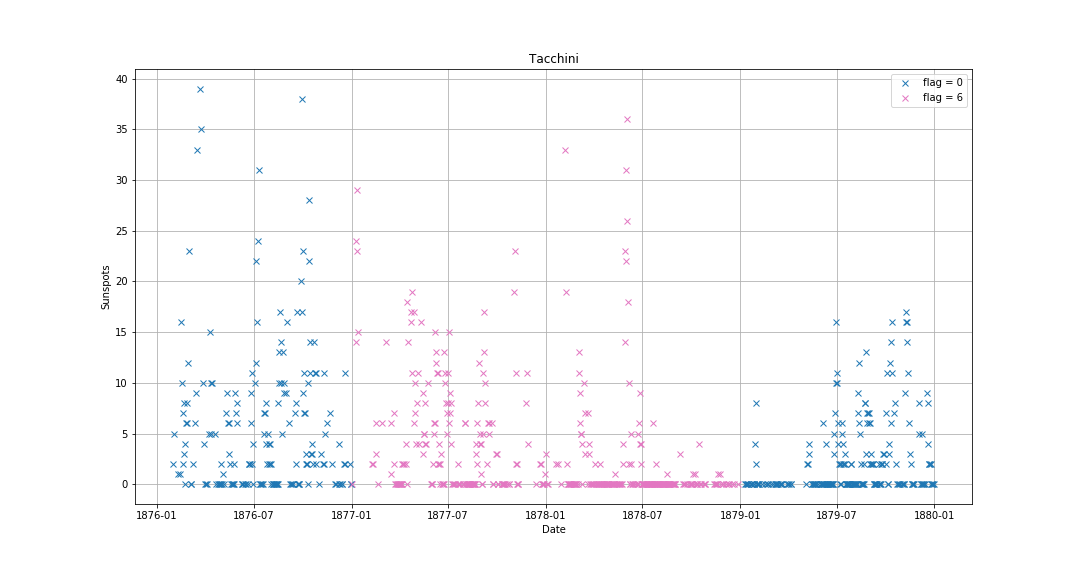
\includegraphics[width=0.5\linewidth]{tacchini1877_patch.png}
    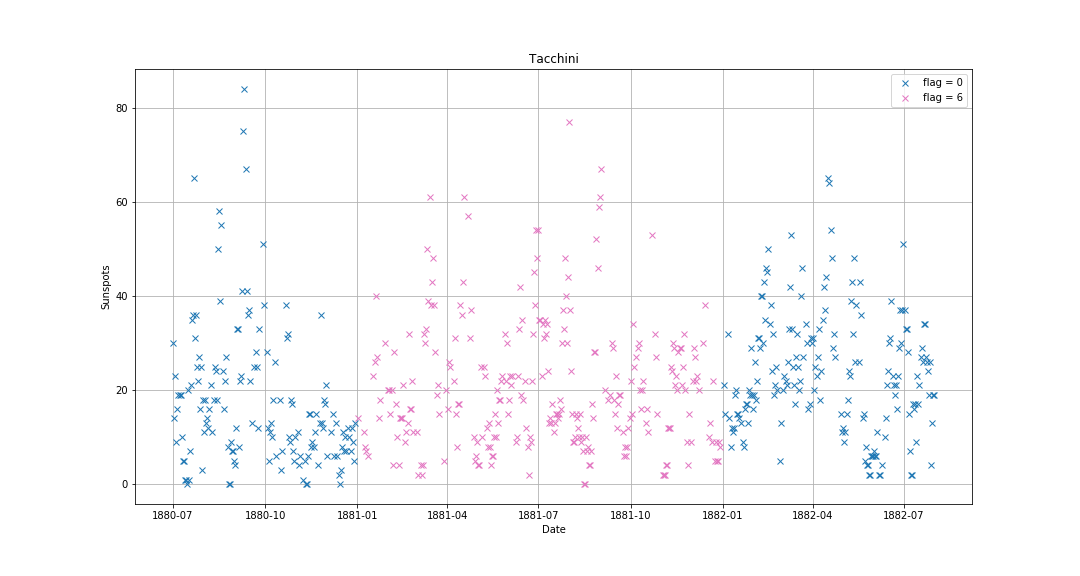
\includegraphics[width=0.5\linewidth]{tacchini1881_patch.png}
    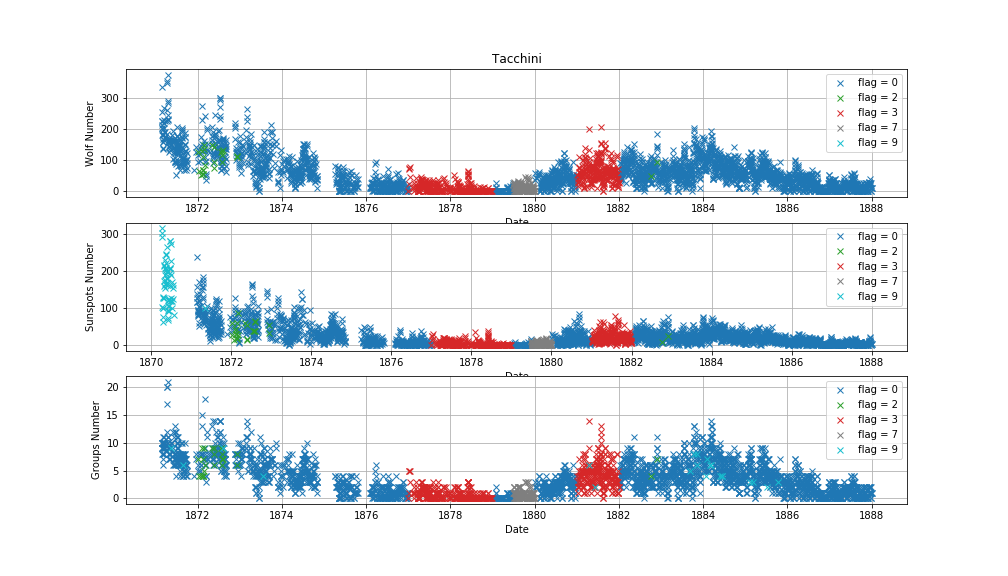
\includegraphics[width=\linewidth]{tacchini_pached.png}
    \caption{Tacchini}
    \label{fig:tacchini}
\end{figure}

\begin{figure}[H]
  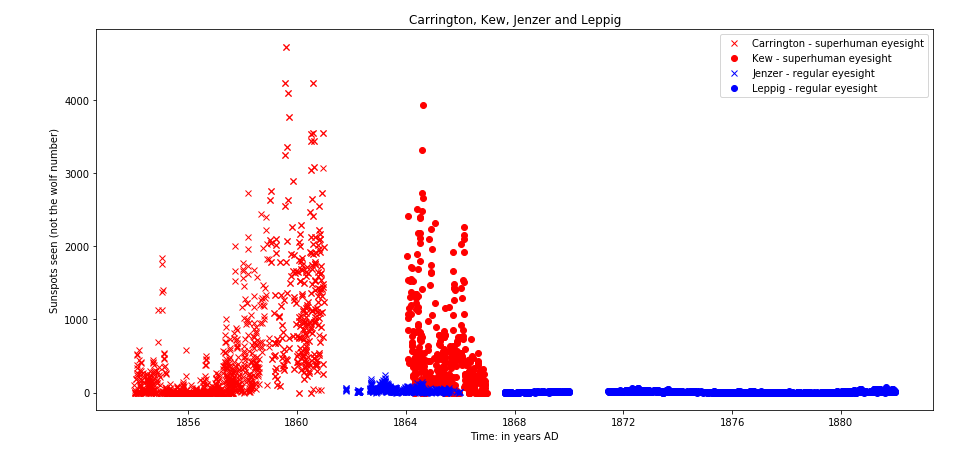
\includegraphics[width=0.93\linewidth]{CarringtonHasGoodEyesight.png}
  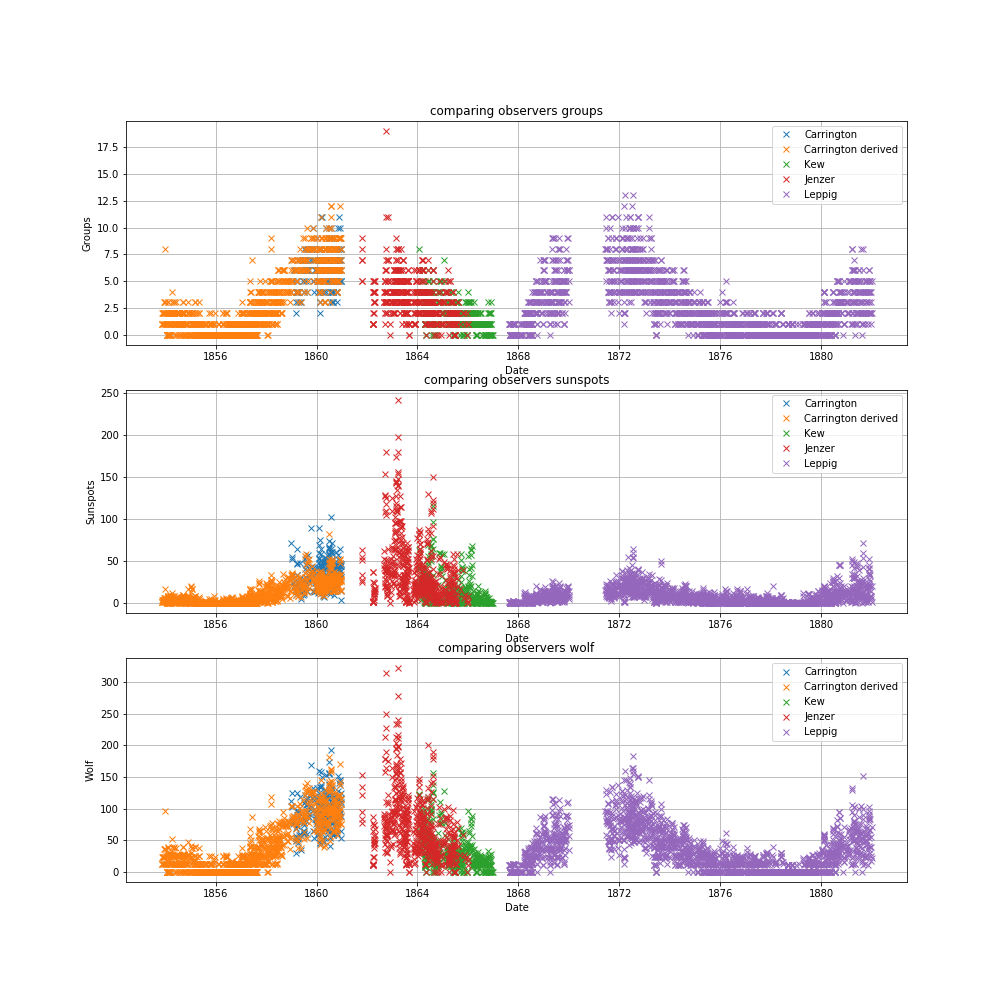
\includegraphics[width=0.9\linewidth]{carrington_kew_after_fix.png}
  \caption{Carrington and Kew - input penumbras instead of sunspots}
  \label{fig:carrington-kew-penumbras}
\end{figure}

\begin{figure}[H]
    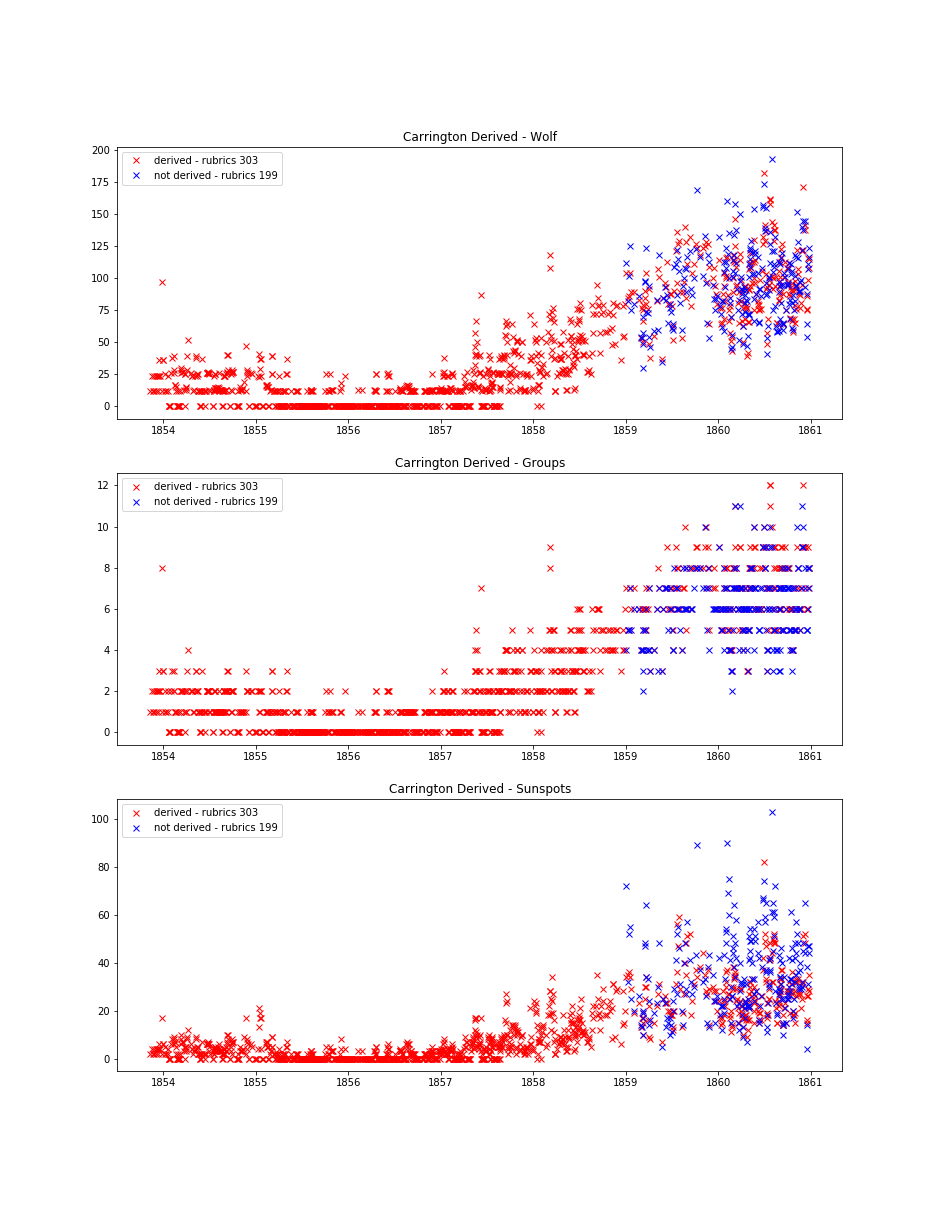
\includegraphics[width=\linewidth]{carrington_derived.png}
    \caption{Carrington derived}
    \label{fig:carrington_derived}
\end{figure}

\begin{figure}[H]
    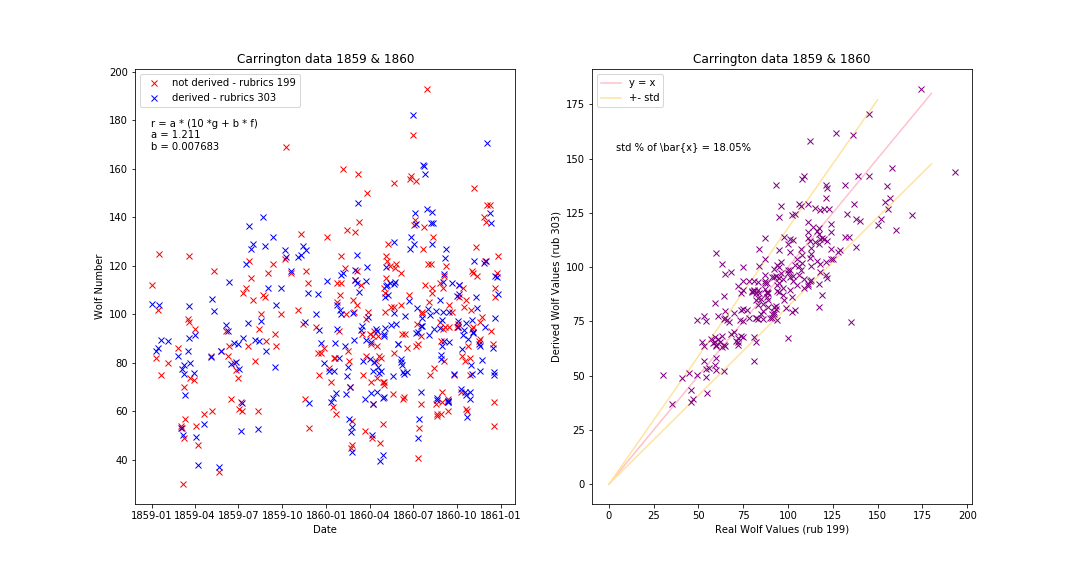
\includegraphics[width=\linewidth]{carrington_fit_wolf.png}
    \caption{Carrington wolf fit}
    \label{fig:carrington_fit_wolf}
\end{figure}

\begin{figure}[H]
    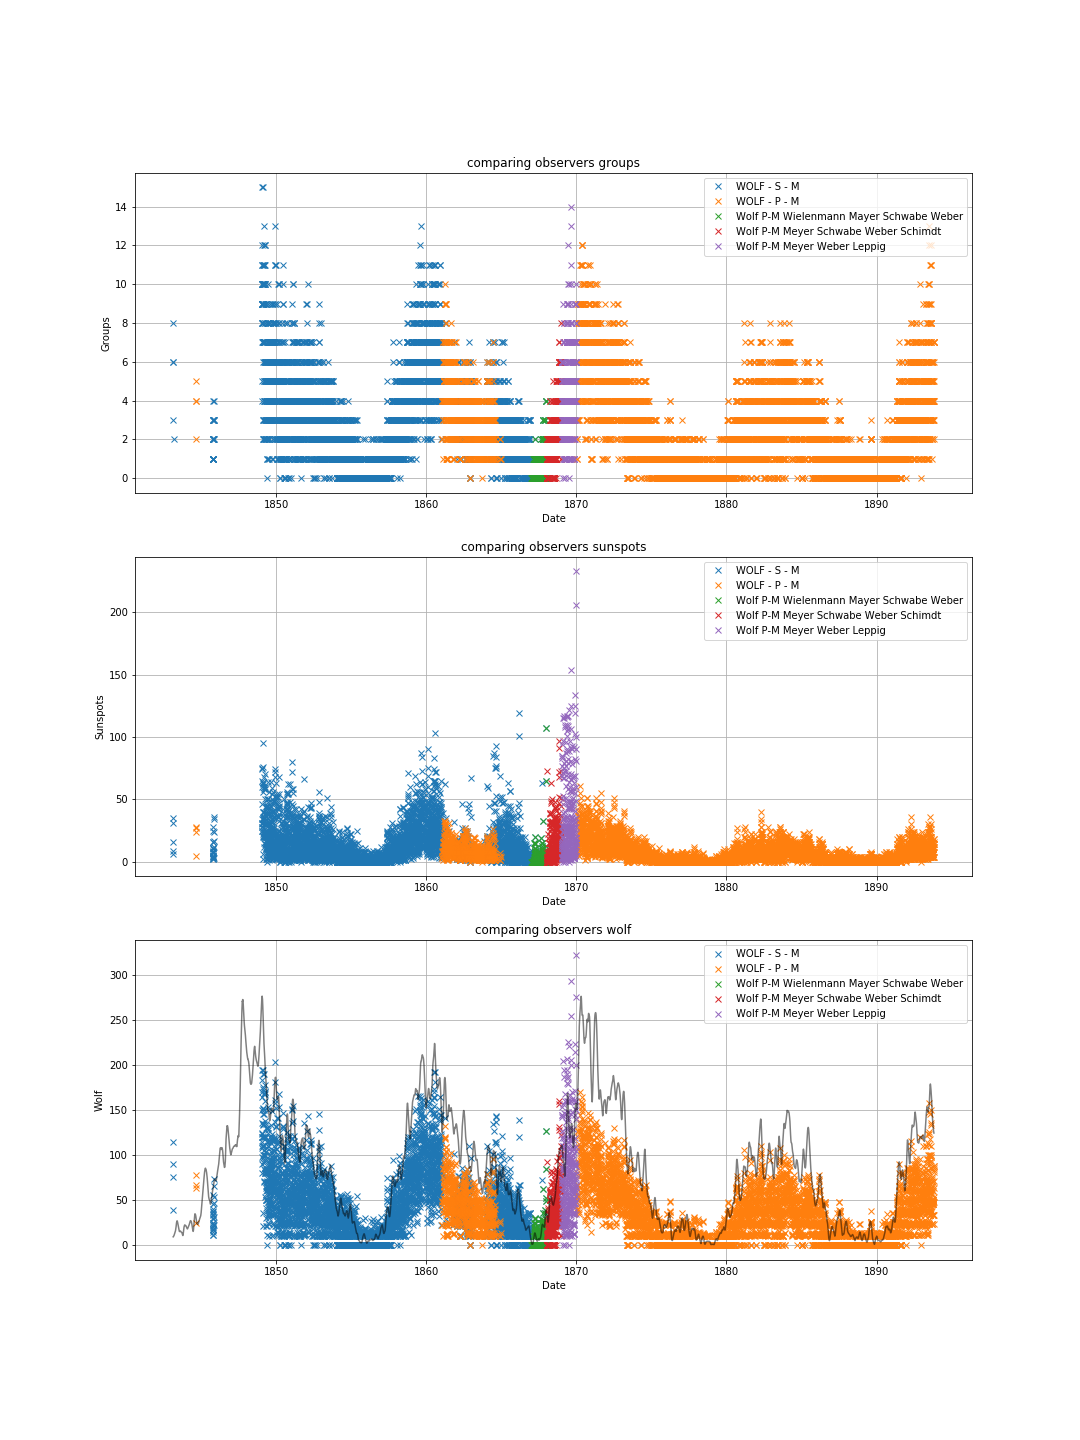
\includegraphics[width=0.5\linewidth]{wolf_comparisons.png}
    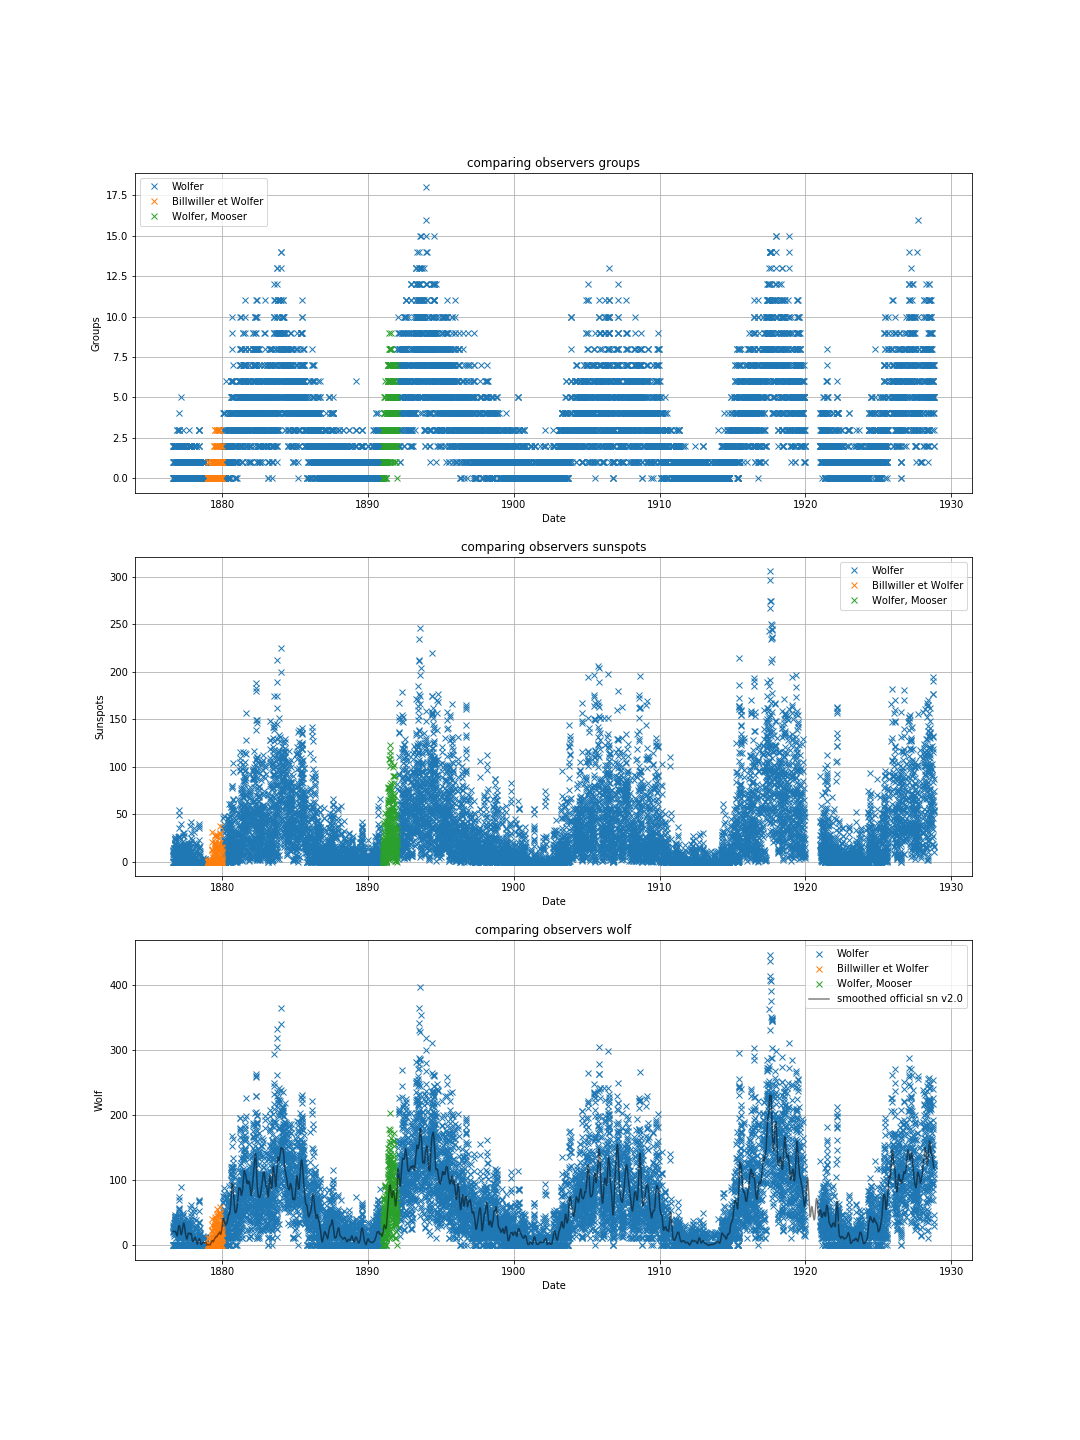
\includegraphics[width=0.5\linewidth]{wolfer_comparisons.png}
    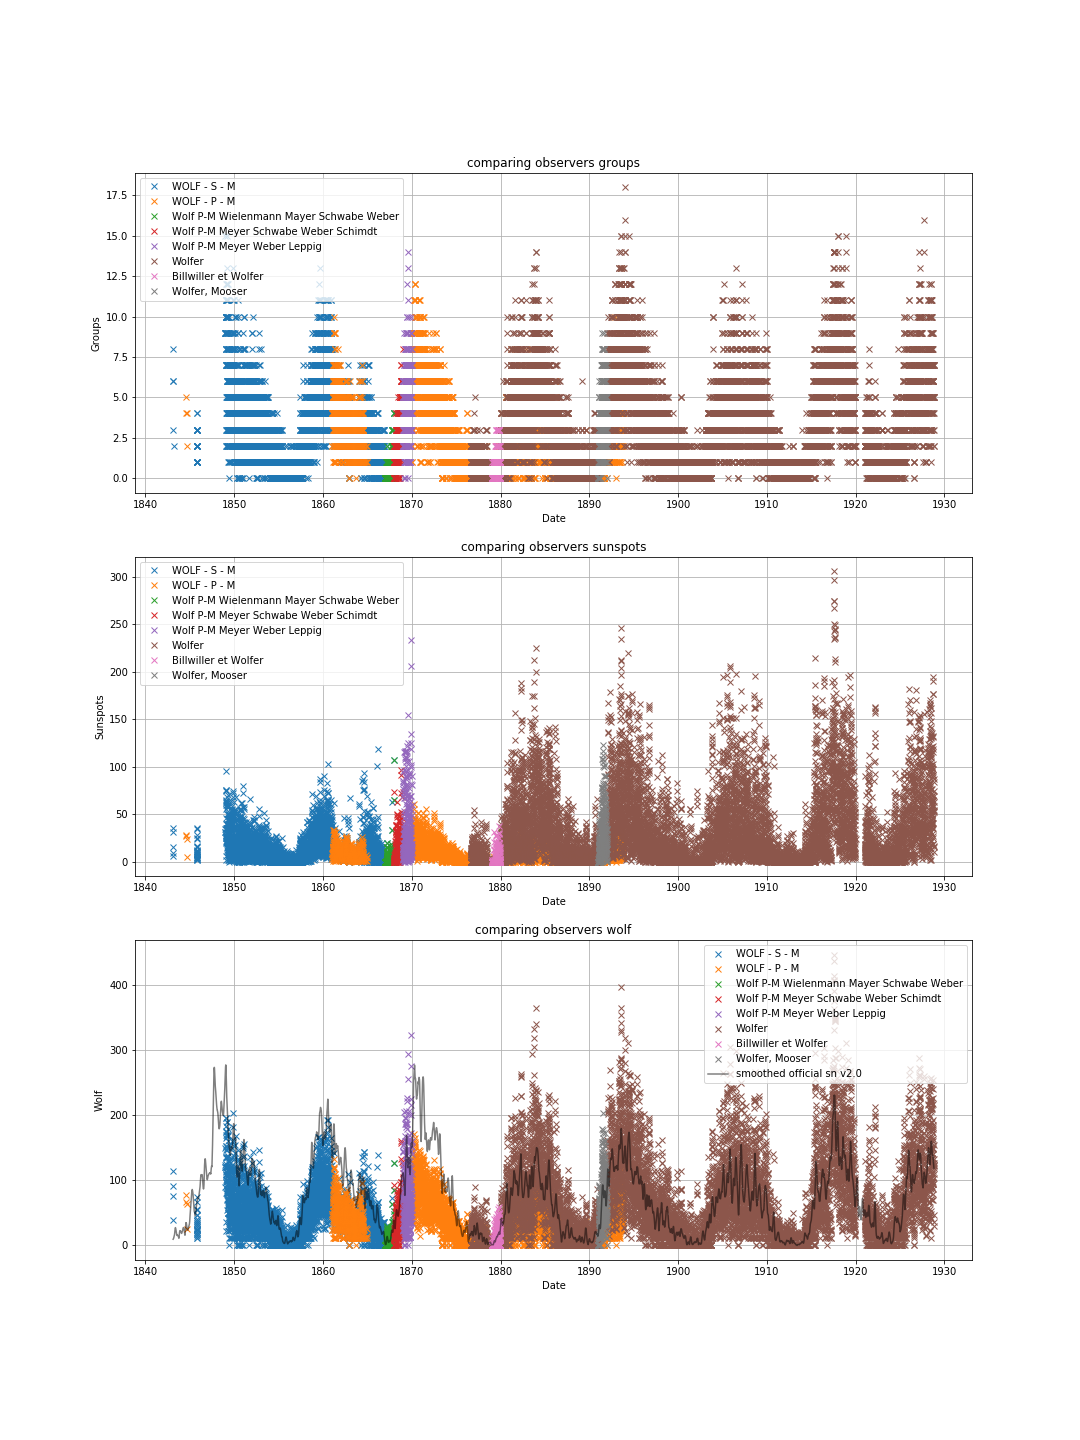
\includegraphics[width=0.5\linewidth]{wolf_and_wolfer_comparisons.png}
    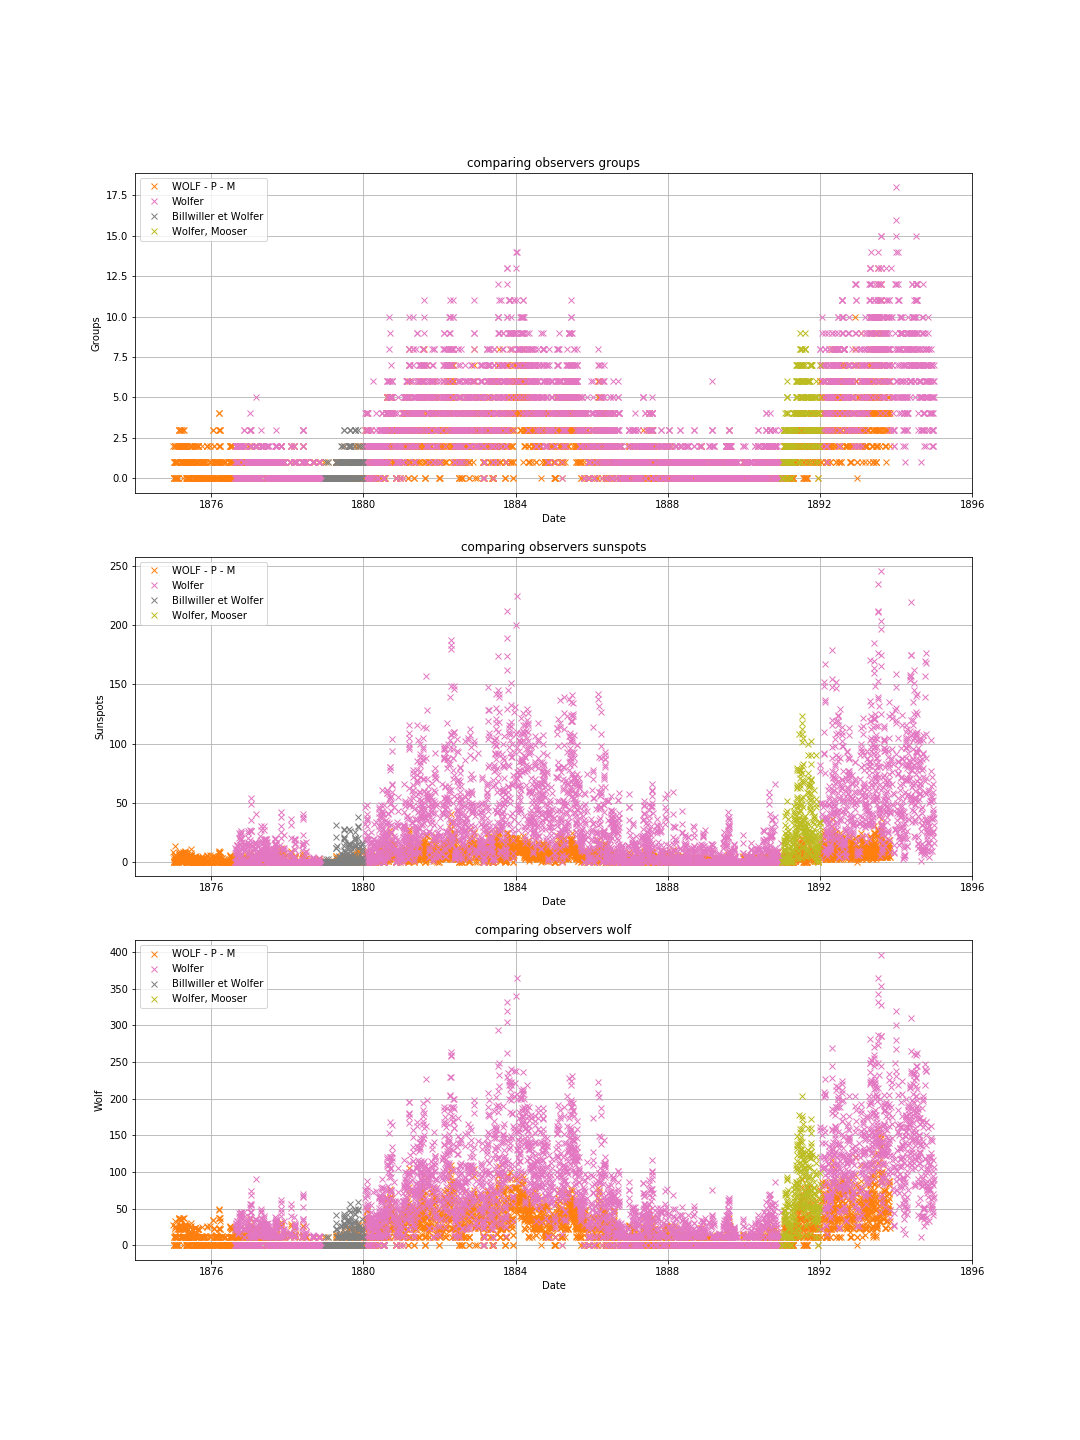
\includegraphics[width=0.5\linewidth]{wolf_and_wolfer_overlap.png}
    \caption{tl = wolf ; tr = wolfer ; bl = wolf and wolfer ; br overlap}
    \label{fig:wolf and wolfer initial plots}
\end{figure}

\section{Conclusions}

\subsection{Before and After - outline of the modifications I made to the database}

\subsection{Problems that remain with the database}

This idea will probably never come to fluition - in the spirit of Herr Wolf who was the first one to estimate $\pi$ by monte-carlo approximation, find the frequency of random errors in the Mittheilungen by Monte-Carlo approximation (should take about 1 day). Pick 1000 to 2000 datapoints at random using some algorythem, and find each one in the mittheilungen to see if it is entered correctly, do some stats on this and calculate a student error factor. (better to look up if there are known numbers for this kind of task)

\section{Miscellaneous}

\subsubsection{Thought repository - ideas that may or may not come into fluition depending on how efficiently I work and get things that need to be done done}
\begin{itemize}
    \item make some data visualisations to compare each observer's primary and secondary observing equipment
    \item for each day / month / year find the highest observation and the lowest observations and add it to the graph so that we have like an upper bound and a lower bound. 
    \item figure out how to smooth graphs with matplotlib and make something nice out off the big mess i currently have
    \item pie chart of observers with their number of observations
    \item in the final sunspots number graph cut it into 3 or 4 sections that mark changes in the theory behind sunspots: before wolf ; time where plato's ideas of the sun being a perfect sphere still were around ; 1908 George Ellery Hale discovers the magnetic link (p14 of nature's 3rd cycle) ; 1955 eugene parker's theory (p19 of nature's 3rd cycle) ; Nasa send their probe to near the sun
\end{itemize}

\subsection{Converting the $f$ (`aire')}\label{converting the `aire'}
This section has been moved to the log
\end{document}





